\section{Operação}

A operação consistiu na retirada de dois stoplogs do tipo comporta vagão
utilizando uma viga pescadora para içar os stoplogs e um pórtico rolante, que
atua a viga. Como em UHE Jirau, o pórtico rolante é operado por um técnico, em
uma cabine a 10m do solo com visibilidade para a operação. 

Na cabine, o técnico do pórtico rolante confirma a posição
ideal do pórtico seguindo faixas vermelhas indicativas no solo; um
pano vermelho amarrado no cabo que sustenta a viga indica que a viga está
próxima da profundidade máxima; e o som (ronco) do motor sinaliza a pesca so
stoplog. O engenheiro \renan se posicionou na cabine, ao lado do técnico, e
ficou responsável por lhe mostrar o aplicativo do robô ROSA,
alertando aos eventos: mudança de posição da chave, inclinação, profundidade, e
pesca bem sucedida.

Em solo, dois operadores são necessários para alinhar a viga com a guia e
alertar ao técnico do pórtico o estado da operação. Os engenheiros \estevao e
\sylvain ficaram responsáveis por guiar o umbilical no vão dos stoplogs.

A operação foi realizada com sucesso e o técnico do pórtico apontou os seguintes
aspectos positivos em relação ao aplicativo: noção de profundidade da viga para diminuir
a velocidade quando próximo do stoplog; noção de inclinação da viga e
diminuição da velocidade até a estabilização; pesca bem sucedida garantida pelos
sensores.

Como ponto negativo, o técnico apontou o umbilical, pois não possui carretel e
sua manipulação é complexa.

A desinstalação dos equipamentos e empacotamento do sistema mais umbilical foi
rápida, em torno de uma hora.

\begin{figure}[h]
\centering
	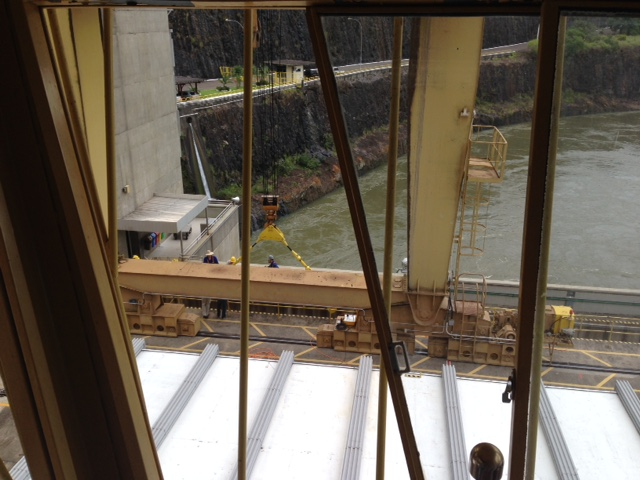
\includegraphics[width=0.9\columnwidth]{figs/IMG_2005.JPG}
	\caption{Vista da cabine do pórtico rolante}
	\label{fig::cabine1}
\end{figure}

\begin{figure}[h]
\centering
	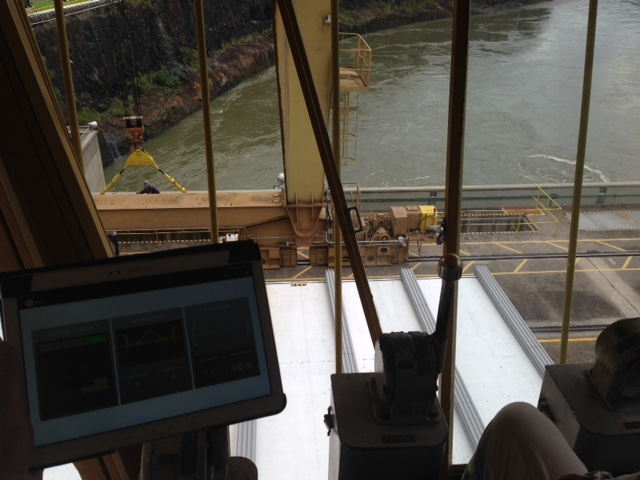
\includegraphics[width=0.9\columnwidth]{figs/IMG_2007.JPG}
	\caption{Vista da cabine do pórtico rolante e tablet}
	\label{fig::cabine2}
\end{figure}